\documentclass[11pt]{article}

\usepackage{sectsty}
\usepackage{graphicx}
\usepackage{hyperref}

% Hyperref
\hypersetup{
    colorlinks=true,
    linkcolor=blue,
    filecolor=magenta,
    urlcolor=cyan,
    pdftitle={Overleaf Example},
    pdfpagemode=FullScreen,
}

% Margins
\topmargin=-0.45in
\evensidemargin=0in
\oddsidemargin=0in
\textwidth=6.5in
\textheight=9.0in
\headsep=0.25in

\title{Automated reasoning project report}
\author{Roberto Tonino}
\date{\today}

\begin{document}
\maketitle


\section{Problem statement}

Delle astronavi aliene sono disposte in modo complanare in modo che possiamo immaginarle nel rettangolo cartesiano (0,0), ($max_x$,0), ($max_x$,$max_y$), (0,$max_y$).
$max_x$ e $max_y$ sono dati di input e vengono anche date le coordinate (intere) delle astronavi presenti. Supponiamo non siano già ad ordinata 0 (ovvero sulla terra).

Ci accorgiamo che ad ogni istante di tempo ogni astronave scende unitariamente (ciascuna componente $y$ cala di 1).

Gli alieni sono ostili e vogliamo fermarli.
Disponiamo di un cannone all'inizio in posizione (0,0) che in un istante di tempo può (1) sparare verticalmente distruggendo la astronave più vicina che si trovi nella stessa ascissa, oppure (2) spostarsi (senza sparare) in un'altra ascissa.
Il tempo per spostarsi di 1,2,3,4, etc caselle sull'asse $x$ è sempre unitario.

Si vuole trovare un piano (se esiste) per evitare che anche solo una astronave tocchi terra.

P.S. \'E possibile ci sia una soluzione furba, ad-hoc, per il problema.
Non cerchiamo quella.
Vogliamo codificarlo e fare risolvere al CP solver o al ASP solver.

\section{Clingo model}

In the first few lines we find the domain predicates.
There are a couple of things to note.
The time/1 predicate started from 0.
This is to indiccate the initial state of the world and means that the model will have t+1 time steps.
The x and y axis also start from 0.
This is because the grid is a cartesian rectangle.
The cannon predicate is arguably the most odd: its' written such that the model can have more than one cannon, but practically the model never takes into account this eventuality.
The cannon predicate comes in this shape in order to be able to use a variable C in further predicates.

The alien/1 predicate comes with an identifier, which is simply an integer counter strarting from 1.

The \texttt{1 { ...  } 1} line is a core part of the model.
it states that for each time step except for the last one the cannon either moes to an X or shots an alien.
The last time step is left our because of how the shoot predicate/action is defined further on: when the cannon shoots, an aliens is considered dead in the next time step.

The ``initial state'' predicate uses the at/4 predicate by positioning the cannon at the coordinates 0,0 as required in the problem statement.

The at/4 predicate is also a core part of the model.
At any fiven time step, it represents the position on the grid of the cannon or of an alien.

The model contains the move, shoot actions.
The move/3 action represents only the movement of the cannon.
The requirement of each alien decreasing its y coordinate at every time step is met via an inertia rule.

The shoot/3 action involves both the cannon and an alien.
The cannon shoots an alien A if at time T their x coordinates are equal.

Additionally, we are enforcing the fact that if the cannon shoots, it will stay in the same position in the next time step

The inertia rules involve aliens.
If, at a ceratin point, an alien is dead it will remain dead and it will preserve its position on the grid.
If an alien is not dead, its y coordinate will decrease at each time step.

The constraints avoid the model to accept a solution where the cannon has a y coordinate different than zero---at each time step.
They also avoid a solution where an alien reaches y=0, which would violate the requirements in the problem statement.


\section{Minizinc model}

In the Minizinc model, we define upfront the variables we need the model to assign values to.
The model represents time steps as array indices.
Like in the clingo model, the move\_x and the shoot variables span in t time steps, compared to t+1 timesteps of the other decision variables.

The plannin concepts of precondition and effect are represented by a conjunction.

The concept of action is represented by a quantified boolean formula (QBF): <formula> with A being the set of aliens and T being 0..t timesteps.
The actions are encoded as constraint in the model.

In the model we also find a constraint that enforces, foreach time setep, the move\_x or the shoot actions to not be in their null state.

Inertia rules are represented by a QBF of the form: <formula>.
The idea is to have a if-else-like structure of an imperative programming language.

Finally, the only constraint in the model prohibits the cannon to shoot to teh same alien twice.
This can probably be removed by adding a precondition to the shoot action.


\section{Benchmarks}

\subsection{Instance generation}
Both clingo and minizinc benchmarks were run on 10 instances of aliens.
The instances were generated with the program ``generate.ts'' (included in the zip file) that is run with the command \texttt{bun generate.ts} (it uses \href{https://bun.sh/}{bun}, a modern TypeScript runtime, but can be ran with node.js as well with some additional work).
The program contains 3 variables: \texttt{x}, \texttt{y} and \texttt{numberOfAliens}.

The $y$ coordinates of the aliens are generated by taking the variable \texttt{y} and decreasing it for each alien present in the instance, obtaining a sequence that starts at $y - 1$ and ends at $y - numberOfAliens$.
The $x$ coordinates of the aliens are randomly generated between 0 and the variable \texttt{x}.
This way of generating the coordinates ensures that there won't be two aliens in the same position.

It is worth noting that if the variable \texttt{y} is smaller than $2*numberOfAliens$, the model will most likely be unsatisfiable because the cannon won't be able to kill all the aliens before they reach the $0$ coordinate.
The combination of shoot and move takes 2 time steps.
So, if there are 50 aliens all with different x, 100 time steps are required for the cannon to kill all the aliens before they reach 0.
To enable that, the aliens need to be in a high-enough $y$ coordinate to not reach 0.

\subsection{Minizinc instances}

The ``generate.ts'' file generates instances suitable to be used with clingo.
A combination of a shell script, a TypeScript script and a manual step are used to convert them to Minizinc instances.
The two scripts can be found in the zip file and are named \texttt{minizinc/convert} and \texttt{minizinc/convert.ts} respectively.
The \texttt{convert} script creates 10 files names \texttt{aliens.1.mzn}, \texttt{aliens2.mzn}, etc.
The files contain two arrays which values are extracted from \texttt{clingo/aliens1.lp}, \texttt{clingo/aliens2.lp}, etc.
The manual step consists in adding four integer parameters to the files.
The four integer parameters are: \texttt{t}, \texttt{mx} ($max_x$), \texttt{my} ($max_y$), and \texttt{a} (number of aliens).

\subsection{Benchmark setup}

Every instance is ran 10 times with 3 warmup runs.
The clingo model was ran with three different configurations: ``auto'', ``jumpy'', and ``trendy''.
The Minizinc model was ran with two different solvers: default, and ``chuffed''.

The results---in JSON format---are stored in the \texttt{clingo/benchmarks} and \texttt{minizinc/benchmarks}.

\subsection{Clingo model}

From the benchmarks the ``jumpy'' configuration is overall the fastest for this problem.
In \autoref{fig:clingo-bench-comparative} a visualization of the results is presented.
On the x axis there are the 10 aliens files, while on the y acis the runtime of the benchmarks.
There are 3 bars for each file representing the 3 different configurations.

In \autoref{table:clingo-bench-comparative} the full benchmark results is presented.
The raw data can be found in \texttt{clingo/benchmarks}.

\begin{figure}[]
  \centering
  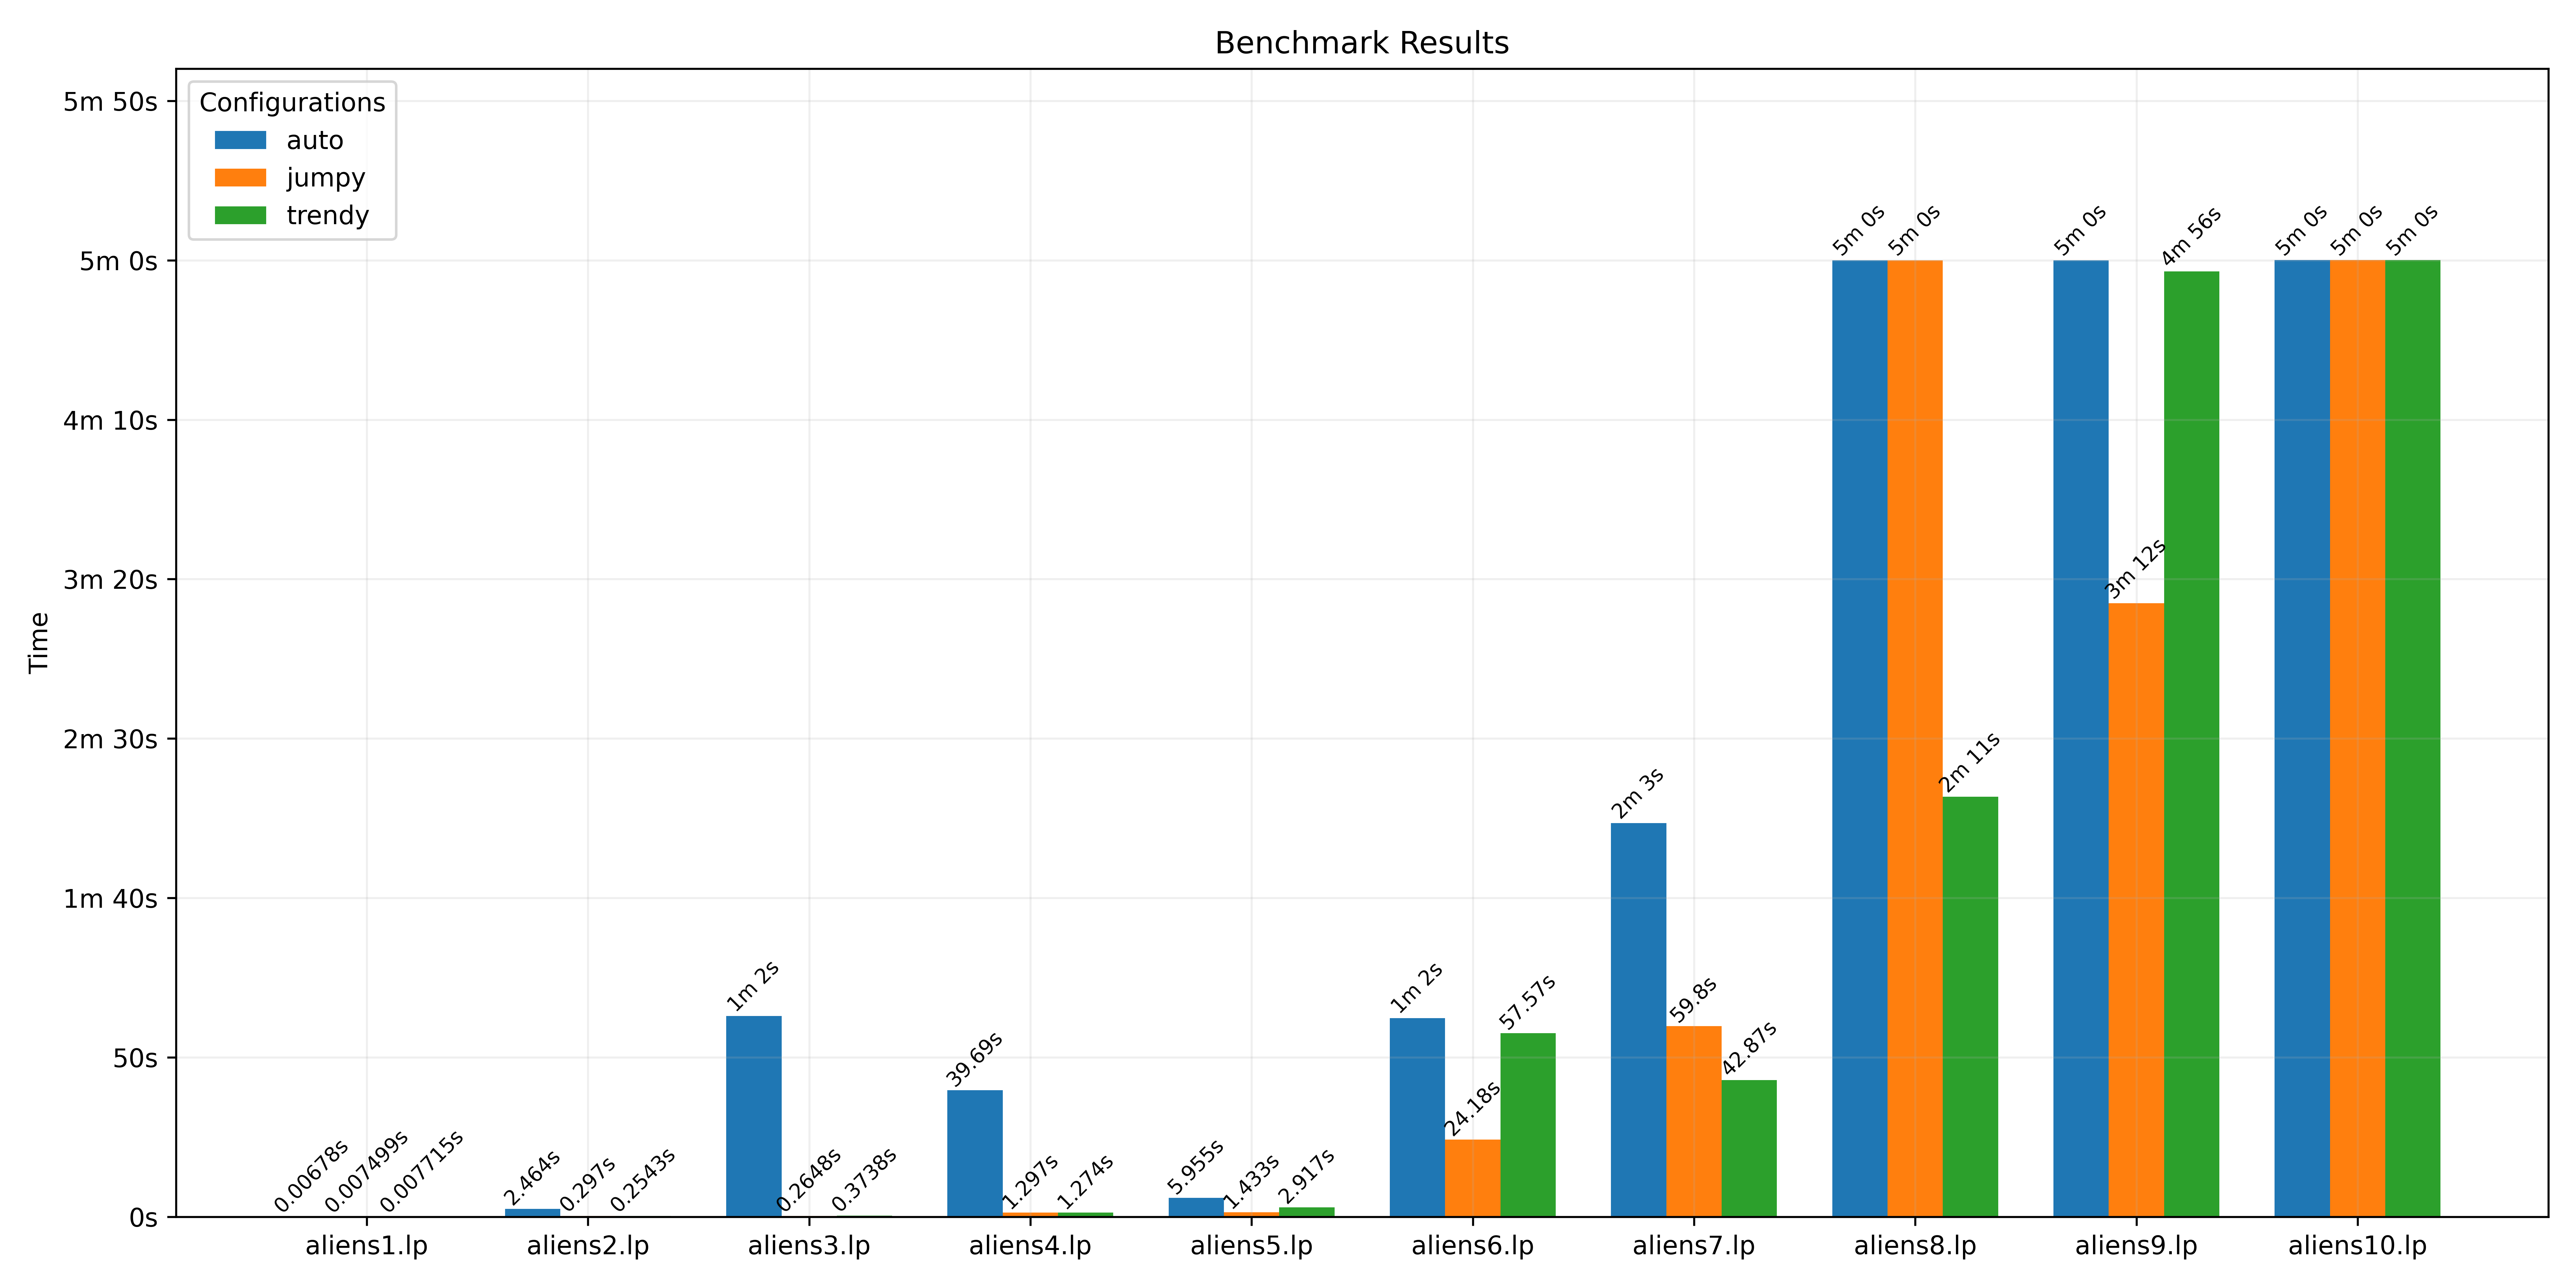
\includegraphics[width=\textwidth]{./clingo/benchmarks/comparative.png}
  \caption{Comparing clingo benchmark results}
  \label{fig:clingo-bench-comparative}
\end{figure}

\begin{table}[h]
  \centering
  \begin{tabular}{|llrrrrrr|}
    \hline
    Aliens & Configuration & Mean & Std Dev & Min & Max & Times faster & Percentage \\
    \hline
    aliens1 & auto & 0.0068~s & 0.0014~s & 0.005~s & 0.0091~s & 1.0x & baseline \\
    & jumpy & 0.0075~s & 0.0014~s & 0.006~s & 0.01~s & 0.9x & +10.61\% \\
    & trendy & 0.0077~s & 0.0015~s & 0.0057~s & 0.01~s & 0.9x & +13.79\% \\
    \hline
    aliens2 & auto & 2.46~s & 0.023~s & 2.43~s & 2.50~s & 1.0x & baseline \\
    & jumpy & 0.3~s & 0.023~s & 0.28~s & 0.34~s & 8.3x & -87.95\% \\
    & trendy & 0.25~s & 0.024~s & 0.23~s & 0.31~s & 9.7x & -89.68\% \\
    \hline
    aliens3 & auto & 62.98~s & 0.8~s & 61.96~s & 63.94~s & 1.0x & baseline \\
    & jumpy & 0.26~s & 0.024~s & 0.23~s & 0.3~s & 237.9x & -99.58\% \\
    & trendy & 0.37~s & 0.026~s & 0.31~s & 0.4~s & 168.5x & -99.41\% \\
    \hline
    aliens4 & auto & 39.69~s & 0.51~s & 38.94~s & 40.33~s & 1.0x & baseline \\
    & jumpy & 1.30~s & 0.053~s & 1.24~s & 1.41~s & 30.6x & -96.73\% \\
    & trendy & 1.27~s & 0.069~s & 1.22~s & 1.46~s & 31.2x & -96.79\% \\
    \hline
    aliens5 & auto & 5.96~s & 0.16~s & 5.86~s & 6.39~s & 1.0x & baseline \\
    & jumpy & 1.43~s & 0.17~s & 1.32~s & 1.79~s & 4.2x & -75.93\% \\
    & trendy & 2.92~s & 0.098~s & 2.84~s & 3.18~s & 2.0x & -51.02\% \\
    \hline
    aliens6 & auto & 62.34~s & 0.28~s & 61.96~s & 62.73~s & 1.0x & baseline \\
    & jumpy & 24.18~s & 0.31~s & 23.79~s & 24.76~s & 2.6x & -61.22\% \\
    & trendy & 57.57~s & 0.99~s & 56.38~s & 59.26~s & 1.1x & -7.65\% \\
    \hline
    aliens7 & auto & 123.48~s & 1.30~s & 121.94~s & 125.81~s & 1.0x & baseline \\
    & jumpy & 59.80~s & 0.67~s & 59.00~s & 61.23~s & 2.1x & -51.57\% \\
    & trendy & 42.87~s & 0.56~s & 42.07~s & 43.71~s & 2.9x & -65.28\% \\
    \hline
    aliens8 & auto & 300.01~s & 0.0028~s & 300.01~s & 300.02~s & 1.0x & baseline \\
    & jumpy & 300.01~s & 0.00075~s & 300.00~s & 300.01~s & 1.0x & -0.00\% \\
    & trendy & 131.77~s & 2.80~s & 128.71~s & 136.63~s & 2.3x & -56.08\% \\
    \hline
    aliens9 & auto & 300.01~s & 0.0023~s & 300.01~s & 300.02~s & 1.0x & baseline \\
    & jumpy & 192.42~s & 0.92~s & 191.25~s & 194.26~s & 1.6x & -35.86\% \\
    & trendy & 296.51~s & 1.66~s & 294.17~s & 300.11~s & 1.0x & -1.17\% \\
    \hline
    aliens10 & auto & 300.08~s & 0.035~s & 300.06~s & 300.17~s & 1.0x & baseline \\
    & jumpy & 300.05~s & 0.0036~s & 300.05~s & 300.06~s & 1.0x & -0.01\% \\
    & trendy & 300.06~s & 0.014~s & 300.04~s & 300.10~s & 1.0x & -0.00\% \\
    \hline
  \end{tabular}
  \caption{Complete clingo benchmark results}
  \label{table:clingo-bench-comparative}
\end{table}


\end{document}
